% =====================================================================
%  Analysis of Algorithms - Lab 07
%  Gaussian Elimination, Heaps, and LU Decomposition
% =====================================================================
\documentclass[12pt,a4paper]{article}

% ----- Encoding & Language -------------------------------------------
\usepackage[utf8]{inputenc}
\usepackage[T1]{fontenc}
\usepackage[english]{babel}

% ----- Page layout ---------------------------------------------------
\usepackage{geometry}
\geometry{top=2.5cm,bottom=2.5cm,left=2.8cm,right=2.8cm}

% ----- Math ----------------------------------------------------------
\usepackage{amsmath,amssymb,amsthm}
\usepackage{mathtools}

% ----- Code listings -------------------------------------------------
\usepackage{listings}
\usepackage[dvipsnames]{xcolor}

% ----- Graphics & floats ---------------------------------------------
\usepackage{graphicx}
\usepackage{float}
\usepackage{tikz}
\usetikzlibrary{arrows.meta, positioning, shapes.geometric, calc}

% ----- Tables --------------------------------------------------------
\usepackage{booktabs}
\usepackage{array}
\usepackage{multirow}

% ----- Layout helpers ------------------------------------------------
\usepackage{enumitem}
\usepackage{fancyhdr}
\setlength{\headheight}{25pt}
\usepackage{titlesec}
\usepackage{parskip}
\usepackage{mdframed}
\usepackage{caption}
\usepackage{subcaption}
\usepackage{setspace}
\usepackage{hyperref}
\hypersetup{colorlinks=true,linkcolor=NavyBlue,urlcolor=NavyBlue,citecolor=NavyBlue}

% =====================================================================
%  Colour palette
% =====================================================================
\definecolor{primary}{RGB}{20,60,120}
\definecolor{accent}{RGB}{0,120,180}
\definecolor{lightbg}{RGB}{247,249,252}
\definecolor{codebg}{RGB}{245,245,245}
\definecolor{codegreen}{RGB}{30,130,30}
\definecolor{codegray}{RGB}{120,120,120}
\definecolor{codepurple}{RGB}{130,0,160}
\definecolor{codeblue}{RGB}{0,0,200}
\definecolor{outputbg}{RGB}{240,248,240}
\definecolor{outputborder}{RGB}{100,160,100}
\definecolor{warningbg}{RGB}{255,250,230}
\definecolor{warningborder}{RGB}{200,160,40}

% =====================================================================
%  Listings style
% =====================================================================
\lstdefinestyle{cstyle}{
  language=C,
  backgroundcolor=\color{codebg},
  commentstyle=\color{codegreen}\itshape\small,
  keywordstyle=\color{codeblue}\bfseries,
  numberstyle=\tiny\color{codegray},
  stringstyle=\color{codepurple},
  basicstyle=\ttfamily\footnotesize,
  breakatwhitespace=false,
  breaklines=true,
  captionpos=b,
  keepspaces=true,
  numbers=left,
  numbersep=10pt,
  showstringspaces=false,
  tabsize=4,
  frame=single,
  rulecolor=\color{gray!30},
  xleftmargin=2em,
  framexleftmargin=1.5em,
  aboveskip=8pt,
  belowskip=8pt,
}
\lstset{style=cstyle}

% =====================================================================
%  Theorem environments
% =====================================================================
\theoremstyle{plain}
\newtheorem{theorem}{Theorem}[section]
\newtheorem{lemma}[theorem]{Lemma}
\newtheorem{corollary}[theorem]{Corollary}
\theoremstyle{definition}
\newtheorem{definition}{Definition}[section]
\theoremstyle{remark}
\newtheorem*{remark}{Remark}
\newtheorem*{note}{Note}

% =====================================================================
%  Framed environments
% =====================================================================
\newmdenv[backgroundcolor=outputbg,linecolor=outputborder,linewidth=1.5pt,
 leftmargin=0pt,rightmargin=0pt,innerleftmargin=10pt,innerrightmargin=10pt,
 innertopmargin=6pt,innerbottommargin=6pt,skipabove=8pt,skipbelow=8pt]{outputbox}
\newmdenv[backgroundcolor=warningbg,linecolor=warningborder,linewidth=1.5pt,
 leftmargin=0pt,rightmargin=0pt,innerleftmargin=10pt,innerrightmargin=10pt,
 innertopmargin=6pt,innerbottommargin=6pt,skipabove=8pt,skipbelow=8pt]{keybox}
\newmdenv[backgroundcolor=lightbg,linecolor=primary!40,linewidth=1pt,
 leftmargin=0pt,rightmargin=0pt,innerleftmargin=10pt,innerrightmargin=10pt,
 innertopmargin=6pt,innerbottommargin=6pt,skipabove=6pt,skipbelow=6pt]{infobox}

% =====================================================================
%  Header / footer
% =====================================================================
\pagestyle{fancy}
\fancyhf{}
\fancyhead[L]{\small\color{primary}\textbf{Analysis of Algorithms} \textbar\ Lab 07}
\fancyhead[R]{\small\color{primary}Yachay Tech University}
\fancyfoot[C]{\small\thepage}
\renewcommand{\headrulewidth}{0.5pt}
\renewcommand{\headrule}{\hbox to\headwidth{\color{primary!50}\leaders\hrule height \headrulewidth\hfill}}

% =====================================================================
%  Section formatting
% =====================================================================
\titleformat{\section}{\Large\bfseries\color{primary}}
  {\color{accent}Exercise \thesection.}{0.6em}{}
  [{\vspace{2pt}\color{primary!40}\titlerule[0.8pt]\vspace{4pt}}]
\titleformat{\subsection}{\bfseries\color{primary!80}}{\thesubsection}{0.5em}{}
\titleformat{\subsubsection}{\bfseries\color{primary!60}\itshape}{\thesubsubsection}{0.5em}{}

% =====================================================================
%  Convenience commands
% =====================================================================
\newcommand{\bigO}[1]{\ensuremath{\mathcal{O}(#1)}}
\newcommand{\DAG}{\textsc{dag}}

\begin{document}

% ----------------------- Compact report header -----------------------
\thispagestyle{fancy}
\noindent{\color{primary!35}\rule{\textwidth}{0.4pt}}
\vspace{0.35cm}

\noindent\begin{minipage}[c]{0.23\textwidth}
  
\includegraphics[width=\linewidth]{figures/logo1.png}
\end{minipage}\hfill
\begin{minipage}[c]{0.48\textwidth}
  \centering
  {\large\bfseries\color{primary}YACHAY TECH UNIVERSITY}\\[-1pt]
  {\small\bfseries School of Mathematical and Computational Sciences}\\[2pt]
  {\small\color{primary}Course: Analysis of Algorithms \textbar\ Lab 07}
\end{minipage}\hfill
\begin{minipage}[c]{0.23\textwidth}
  
\includegraphics[width=\linewidth]{figures/logo2.png}
\end{minipage}

\vspace{0.22cm}
\noindent{\color{primary}\rule{\textwidth}{1.2pt}}

\begin{center}
  \vspace{0.18cm}
  {\Large\bfseries\color{primary}Assignment 07: Gaussian Elimination, Heaps,\\[-1pt]
  and LU Decomposition}\\[0.22cm]
  {\small\textbf{Author:} Darío Pomasqui \quad\textbar\quad \textbf{Date:} October 19, 2026}\\[0.10cm]
  {\small\textbf{GitHub Repository:}}\\[-1pt]
  {\footnotesize\url{https://github.com/darioxx32/Algorithm-analysis/tree/main/Deber7}}
\end{center}
\vspace{0.1cm}
\noindent{\color{primary!35}\rule{\textwidth}{0.4pt}}
\vspace{0.35cm}

\begin{abstract}
This report develops and analyzes the four algorithms requested in Assignment 07. The first program converts an augmented matrix to upper-triangular form by Gaussian forward elimination with partial pivoting. The second solves an upper-triangular system by backward substitution and derives its quadratic running time. The third transforms an arbitrary array into a max-heap using bottom-up heap construction. The fourth derives an LU factorization from Gaussian elimination, including row permutations, and solves a linear system using forward and backward substitution. The C programs were compiled with GCC under C11 with warnings enabled; console captures record the resulting program executions.
\end{abstract}

\begin{infobox}
\textbf{Conventions.} Matrices are indexed from zero in C and from one in the mathematical notation when convenient. The linear-system examples use the same system
\[
\begin{aligned}
2x+y-z&=8,\\
-3x-y+2z&=-11,\\
-2x+y+2z&=-3,
\end{aligned}
\qquad\text{whose solution is }(x,y,z)=(2,3,-1).
\]
Using the same input in Exercises 1, 2, and 4 makes it possible to compare the triangular system, its back-substitution result, and the LU solve.
\end{infobox}

\section{Forward elimination for Gaussian elimination}
\subsection{Goal and mathematical operation}
For a system $Ax=b$, Gaussian elimination applies elementary row operations to the augmented matrix $[A\mid b]$ until it is upper triangular. At pivot column $k$, let $p$ be the selected pivot row. For each row $i>k$, define the multiplier
\[
m_{ik}=\frac{a_{ik}}{a_{kk}}.
\]
Subtracting $m_{ik}$ times row $k$ from row $i$ changes the entries by
\[
a_{ij}\leftarrow a_{ij}-m_{ik}a_{kj},\qquad j=k+1,\ldots,n,
\]
where the last column is the right-hand side. This makes the entry below the pivot zero while preserving the solution set, provided the same operation is performed on the augmented column.

\subsection{Pivoting and implementation}
The program uses partial pivoting: among rows $k$ through $n-1$, it picks the row whose entry in column $k$ has the largest absolute value, then swaps that row with row $k$. This avoids dividing by a zero pivot whenever a valid pivot exists and generally reduces numerical error compared with always using the diagonal row. A tolerance of $10^{-12}$ is used to detect a pivot too close to zero for this small demonstration. If no usable pivot exists, the program reports that a unique solution cannot be obtained.

For the sample matrix, the first pivot is $-3$, since it has the greatest magnitude in the first column. The first elimination step removes the $-2$ and $2$ entries below it; after the next pivot step the output is an upper-triangular system. Forward elimination costs $\Theta(n^3)$ arithmetic operations for a dense $n\times n$ system: there are $O(n)$ pivot columns, $O(n)$ rows below each pivot, and up to $O(n)$ entries updated in each row. The matrix is stored in-place, so the auxiliary storage beyond the input is $O(1)$ (the input itself occupies $O(n^2)$).

\begin{keybox}
\textbf{Correctness invariant.} At the start of iteration $k$, all entries below the diagonal in columns $0,\ldots,k-1$ are zero. Eliminating column $k$ preserves those earlier zeros and makes all entries below the new pivot zero. Thus, after the final pivot column, the coefficient matrix is upper triangular and the row operations have preserved the solutions of the original system.
\end{keybox}

\lstinputlisting[style=cstyle,caption={gaussian.c: forward elimination with partial pivoting}]{gaussian.c}
\begin{figure}[H]\centering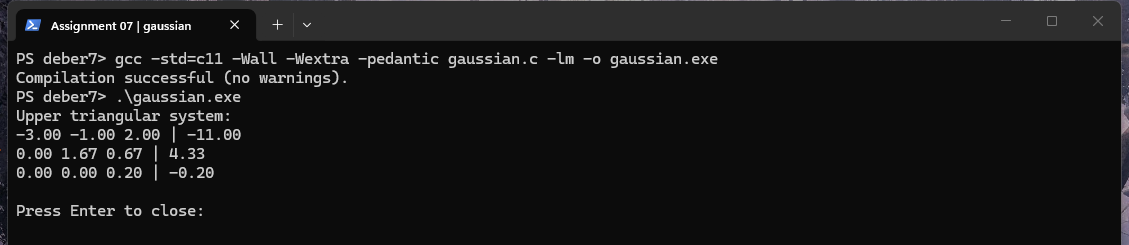
\includegraphics[width=.96\linewidth]{figures/01_gaussian.png}\caption{GCC compilation command and subsequent execution of \texttt{gaussian.exe}; the output is the upper-triangular augmented system.}\end{figure}

\section{Backward substitution and its running time}
\subsection{Algorithm}
After forward elimination, the system has the form $Ux=c$, where $U$ is upper triangular. The last equation contains only $x_{n-1}$, so solve it first and then proceed upward:
\[
x_i=\frac{c_i-\displaystyle\sum_{j=i+1}^{n-1}u_{ij}x_j}{u_{ii}},
\qquad i=n-1,n-2,\ldots,0.
\]
At each row, all variables with index greater than $i$ have already been computed. The code stores the resulting vector in $x$ and uses the known triangular matrix and right-hand side.

\subsection{Proof of the quadratic running time}
For row $i$, the summation has $n-i-1$ terms. Counting each multiply/subtract pair as constant work, the total work over all rows is
\[
\sum_{i=0}^{n-1}(n-i-1)=\sum_{r=0}^{n-1}r=\frac{n(n-1)}{2}.
\]
There are also $n$ divisions and $O(n)$ other operations. Hence the total running time is $\Theta(n^2)$, which establishes the requested $O(n^2)$ upper bound. The output vector requires $O(n)$ extra space. The cost assumes every diagonal entry $u_{ii}$ is nonzero; a zero diagonal pivot indicates that the system cannot be solved by this routine without pivoting or further rank analysis.

\begin{outputbox}
For the triangular system in Exercise 1, backward substitution computes $z=-1$ from the last row, then $y=3$, and finally $x=2$. This recovers the solution of the original system.
\end{outputbox}

\lstinputlisting[style=cstyle,caption={back\_substitution.c: solve an upper-triangular system}]{back_substitution.c}
\begin{figure}[H]\centering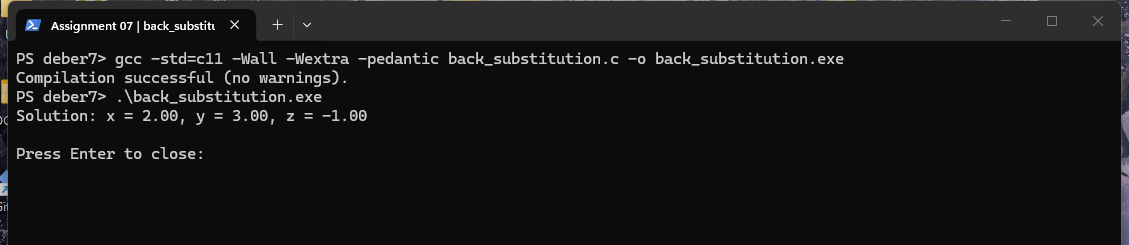
\includegraphics[width=.96\linewidth]{figures/02_back_substitution.png}\caption{GCC compilation command followed by execution of \texttt{back\_substitution.exe} and its solution.}\end{figure}

\section{Transforming an array into a max-heap}
\subsection{Heap property and representation}
A binary max-heap is a complete binary tree in which every parent key is at least as large as either child key. The program stores that tree in an array in level order. With zero-based indexing, node $i$ has left child $2i+1$ and right child $2i+2$. The heap need not be sorted: it only guarantees that the maximum value is at the root and that each parent dominates its children.

\subsection{Bottom-up construction}
Leaves already satisfy the heap property, so the algorithm starts at the last internal node $\lfloor n/2\rfloor-1$ and calls \texttt{heapify} on each node moving toward the root. The iterative \texttt{heapify} compares a node with its children, swaps it with the larger child when needed, and continues down that subtree. When it stops, the subtree rooted at that node is a max-heap. Because children are processed before their parents, each call can rely on both child subtrees already being heaps.

A call to \texttt{heapify} can move down at most the height of the tree, so a single call costs $O(\log n)$. However, applying that bound to all $n/2$ internal nodes would be loose. Nodes close to the leaves have height zero or one, and only a few nodes have large height. The aggregate work is bounded by
\[
\sum_{h=0}^{\lfloor\log_2 n\rfloor} O\!\left(\frac{n}{2^{h+1}}\,h\right)=O(n),
\]
so bottom-up heap construction is linear-time. The iterative procedure uses $O(1)$ auxiliary space in addition to the input array.

\begin{keybox}
\textbf{Result check.} The output array is a valid max-heap when each internal array position is at least as large as its existing children. Its root is the largest array value. The relative order of siblings or of different subtrees is not specified.
\end{keybox}

\lstinputlisting[style=cstyle,caption={heap.c: bottom-up max-heap construction}]{heap.c}
\begin{figure}[H]\centering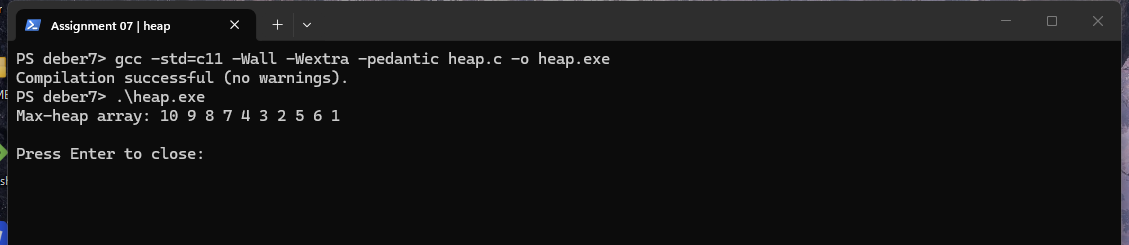
\includegraphics[width=.96\linewidth]{figures/03_heap.png}\caption{GCC compilation command followed by execution of \texttt{heap.exe} and its max-heap array.}\end{figure}

\section{Solving a system using LU decomposition}
\subsection{From elimination to factorization}
Gaussian elimination can be recorded as a factorization instead of discarding the elimination operations. The multipliers used to eliminate entries below each pivot become the subdiagonal entries of a lower-triangular matrix $L$; the final eliminated matrix becomes the upper-triangular matrix $U$. With partial pivoting, row swaps must also be recorded in a permutation matrix $P$, giving
\[
PA=LU.
\]
The diagonal of $L$ is set to one. The equation $Ax=b$ is then transformed by applying $P$:
\[
LUx=Pb.
\]
Define $y=Ux$. First solve $Ly=Pb$ using forward substitution, then solve $Ux=y$ using backward substitution.

\subsection{Row swaps and algorithm details}
In \texttt{lu.c}, the permutation vector records which original row occupies each current row. When a pivot swap occurs, the program swaps rows of the working matrix, swaps already computed entries in the corresponding rows of $L$, and updates the permutation vector. Swapping the previous columns of $L$ is essential: those entries contain multipliers from earlier elimination steps and must follow their rows. The program then performs elimination, storing each multiplier in $L$ and updating the remaining working matrix to form $U$. If a pivot is smaller than the tolerance, it reports a singular matrix.

The factorization takes $\Theta(n^3)$ arithmetic operations for a dense matrix. Once factors are available, each triangular solve takes $\Theta(n^2)$, so solving one system after factorization costs $\Theta(n^3)$ overall. If the same matrix is reused with several right-hand sides, the factorization is done once and each additional solve costs $\Theta(n^2)$. The program requires $O(n^2)$ storage for the matrices and $O(n)$ storage for vectors and the permutation.

\begin{outputbox}
The example's first column causes a pivot-row swap, illustrating why the permutation $P$ is needed. The resulting solution printed by the program is $x_1=2$, $x_2=3$, and $x_3=-1$.
\end{outputbox}

\lstinputlisting[style=cstyle,caption={lu.c: Gaussian-elimination-based $PA=LU$ factorization and solve}]{lu.c}
\begin{figure}[H]\centering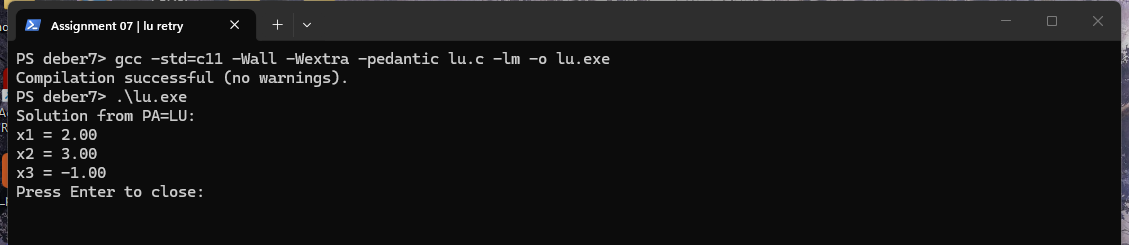
\includegraphics[width=.96\linewidth]{figures/04_lu.png}\caption{GCC compilation command followed by execution of \texttt{lu.exe} and its solution.}\end{figure}

\section*{Compilation, execution, and conclusion}
Each source file is a standalone C11 program. The programs were compiled with GCC using warnings enabled. For example:
\begin{verbatim}
gcc -std=c11 -Wall -Wextra -pedantic gaussian.c -lm -o gaussian.exe
.\gaussian.exe
\end{verbatim}
The \texttt{-lm} library option is required by the programs that use \texttt{fabs}. All four programs compiled without warnings and their outputs are shown in the included console captures. The implementations demonstrate the connections between elimination and triangular solving, the linear construction time of a heap, and the way Gaussian elimination yields an LU factorization. Backward substitution requires quadratic time because its row sums contain $0,1,\ldots,n-1$ terms in total.

\end{document}
